\documentclass[12pt, twoside]{book}

\usepackage[margin=1in]{geometry}
\usepackage[utf8]{inputenc}
\usepackage{verbatim}
\usepackage{pgfplots}
    \pgfplotsset{compat=1.12,}
\usepackage{enumitem}
\usepackage{amsmath,amsfonts,amsthm,amssymb,graphicx,mathtools,hyperref}
\usepackage{wrapfig}
\usepackage[export]{adjustbox}
\usepackage{tikz}
\renewcommand\qedsymbol{$\blacksquare$}
\usetikzlibrary{positioning}
\newcommand{\A}{\mathbb{A}}
\newcommand{\B}{\mathbb{B}}
\newcommand{\C}{\mathbb{C}}
\newcommand{\D}{\mathbb{D}}
\newcommand{\E}{\mathbb{E}}
\newcommand{\F}{\mathbb{F}}
\newcommand{\G}{\mathbb{G}}
\newcommand{\Hb}{\mathbb{H}} %
\newcommand{\I}{\mathbb{I}}
\newcommand{\J}{\mathbb{J}}
\newcommand{\K}{\mathbb{K}}
\newcommand{\Lb}{\mathbb{L}} %
\newcommand{\M}{\mathbb{M}}
\newcommand{\N}{\mathbb{N}}
\newcommand{\Ob}{\mathbb{O}} %
\newcommand{\Pb}{\mathbb{P}} % 
\newcommand{\Q}{\mathbb{Q}}
\newcommand{\R}{\mathbb{R}}
\newcommand{\Sb}{\mathbb{S}} % 
\newcommand{\T}{\mathbb{T}}
\newcommand{\U}{\mathbb{U}}
\newcommand{\V}{\mathbb{V}}
\newcommand{\W}{\mathbb{W}}
\newcommand{\X}{\mathbb{X}}
\newcommand{\Y}{\mathbb{Y}}
\newcommand{\Z}{\mathbb{Z}}
\newcommand{\Ac}{\mathcal{A}}
\newcommand{\Bc}{\mathcal{B}}
\newcommand{\Cc}{\mathcal{C}}
\newcommand{\Dc}{\mathcal{D}}
\newcommand{\Ec}{\mathcal{E}}
\newcommand{\Fc}{\mathcal{F}}
\newcommand{\Gc}{\mathcal{G}}
\newcommand{\Hc}{\mathcal{H}} %
\newcommand{\Ic}{\mathcal{I}}
\newcommand{\Jc}{\mathcal{J}}
\newcommand{\Kc}{\mathcal{K}}
\newcommand{\Lc}{\mathcal{L}} %
\newcommand{\Mc}{\mathcal{M}}
\newcommand{\Nc}{\mathcal{N}}
\newcommand{\Oc}{\mathcal{O}} %
\newcommand{\Pc}{\mathcal{P}} % 
\newcommand{\Qc}{\mathcal{Q}}
\newcommand{\Rc}{\mathcal{R}}
\newcommand{\Sc}{\mathcal{S}} % 
\newcommand{\Tc}{\mathcal{T}}
\newcommand{\Uc}{\mathcal{U}}
\newcommand{\Vc}{\mathcal{V}}
\newcommand{\Wc}{\mathcal{W}}
\newcommand{\Xc}{\mathcal{X}}
\newcommand{\Yc}{\mathcal{Y}}
\newcommand{\Zc}{\mathcal{Z}}
\newcommand{\ita}[1]{\textit{#1}}
\newcommand{\com}[2]{#1\backslash#2}
\newcommand{\oneton}{\{1,2,3,...,n\}}
\newcommand\idea[1]{\begin{gather*}#1\end{gather*}}
\newcommand\ef{\ita{f} }
\newcommand\eff{\ita{f}}
\newcommand\proofs[1]{\begin{proof}#1\end{proof}}
\newcommand\inv[1]{#1^{-1}}
\newcommand\setb[1]{\{#1\}}
\newcommand\en{\ita{n }}
\newcommand{\vbrack}[1]{\langle #1\rangle}
\DeclareMathOperator{\ord}{ord}
\DeclareMathOperator{\re}{Re}
\DeclareMathOperator{\im}{Im}

\theoremstyle{plain}
\newtheorem{theorem}{Theorem}[section]
\newtheorem{axiom}{Axiom}[section]
\newtheorem{lemma}[theorem]{Lemma}
\newtheorem{proposition}[theorem]{Proposition}
\newtheorem{postulate}{Postulate}
\newtheorem*{corollary}{Corollary}

\theoremstyle{plain} % just in case the style had changed
\newcommand{\thistheoremname}{}
\newtheorem*{genericthm}{\thistheoremname}
\newenvironment{namedtheorem}[1]
  {\renewcommand{\thistheoremname}{#1}%
   \begin{genericthm}}
  {\end{genericthm}}

\theoremstyle{definition}
\newtheorem*{definition}{Definition}
\newtheorem{conjecture}{Conjecture}
\newtheorem{example}{Example}[chapter]
\newtheorem*{HW}{Homework}

\theoremstyle{remark}
\newtheorem*{remark}{Remark}
\newtheorem*{claim}{Claim}
\newtheorem*{note}{Note}

\renewcommand*{\proofname}{Proof}



\title{Analysis}
\author{Alec Zabel-Mena\\ \textbf{\underline{Text}} \\Principles of Mathematical 
    Analysis ($3^{rd}$ edition) \\ Walter Rudin}
\date{\today}

\begin{document}

\maketitle

%----------------------------------------------------------------------------------------
%	CHAPTER X
%----------------------------------------------------------------------------------------

\chapter{The Real and Complex Numbers} % Main chapter title

\label{Chapter1} % Change X to a consecutive number; for referencing this chapter elsewhere, use \ref{ChapterX}

%% to include section files use the \input{} command.

%----------------------------------------------------------------------------------------
%	SECTION 3.1
%----------------------------------------------------------------------------------------

\section{Some Elementary Observations} \hspace{10mm}

Consider the equation $x^2-117x+31=0$. We claim that there are no integer solutions to this equation. Let $n$ be an integer
, then $n$ is either even or odd. If $n$ is even, then so is  $n^2$ and  $17n$; hence $x^2-117x+31$ is odd. Likewise if $n$ 
is odd, then so is $n^2$ and  $117n$, thus $x^2-117x+31$ is even and so we see that $x^2-117x+31$ is never $0$.  

%----------------------------------------------------------------------------------------
%	SECTION 1.2
%----------------------------------------------------------------------------------------

\section{The Basis and Subbasis for a Topology.}

\begin{definition}
    If $X$ is a set, the \textbf{basis} for a topology on $X$ is a collection $\Bc$ of 
    subsets of  $X$, called \textbf{basis elements}, such that:
        \begin{enumerate}[label=(\arabic*)]
            \item For every $x \in X$, there is a  $B \in \Bc$ such that $x \in B$.

            \item For $B_1,B_2 \in \Bc$, if $x \in B_1 \cap B_2$, then there is a $B_3 \in \Bc$ 
                such that $x \in B_3 \subseteq B_1 \cap B_2$
        \end{enumerate}
We define the topology $\Tc$ \textbf{generated} by $\Bc$ to be collection of open sets: 
$\Tc=\{U \subseteq X: x \in B \text{ for some } B \in \Bc\}$.
\end{definition}

\begin{theorem}\label{1.2.1}
    Let $X$ be a set, and  $\Bc$ a basis of  $X$, then the collection of subsets 
    of  $X$, $\Tc=\{U \subseteq X: x \in B \text{ for some } B \in \Bc\}$ is a topology on $X$.
\end{theorem}
\begin{proof}
    Let $\Bc$ be a basis for a topology in  $X$, and consider  $\Tc$ as defined 
    above. Cleary, $\emptyset \in X$ and so is  $X$.

    Now let  $\{U_{\alpha}\}$ be a subcollection of subsets of  $X$, and let  $U=\bigcup{U_{\alpha}}$. 
    Then if  $x \in U$ for some  $\alpha$, there is a  $B_{\alpha}$ such that  $x \in B_{\alpha} \subseteq U_{\alpha}$, 
    thus  $x \in B_{\alpha} \subseteq U$.

    Now let  $x \in  U_1 \cap U_2$, and choose $B_1,B_2 \in \Bc$ such that $x \in B_1 \subseteq U_1$ 
    and $x \in B_2 \subseteq U_2$. Then  by definition, there is a $B_3$ for which $x \in B_3 \subseteq B_1 \cap B_2$.
    Now suppose for arbitrary $n$, that  $U=\bigcap_{i=1}^{n}{U_i} \in \Tc$, for some finite 
    subcollection  $\{U_i\}$ of subsets of  $X$. Then by let  $B_n, B_{n+1} \in \Bc$ such that 
    $x \in B_n \subseteq U$ and  $x \in B_{n+1} \subseteq U_{n+1}$. Then by our hypothesis, there is a  $B$ 
for which  $x \in B \subseteq B_n \cap B_{n+1}$, thus  $U \cap U_{n+1}=\bigcap_{i=1}^{n+1}{U_i} \in \Tc$. 
This make $\Tc$ a topology on  $X$.
\end{proof}

\begin{example}
    \begin{enumerate}[label=(\arabic*)]
        \item Let $\Bc$ be the set of all circular regions in the plane  $\R \times \R$, then 
            $\Bc$ satisfies the conditions needed for a basis.

        \item The collection  $\Bc'$ in  $\R \times \R$ of all rectangular region also 
            forms a basis for a topology on  $\R \times \R$.

        \item For any set  $X$, the set of all  $1$-point elements of  $X$ forms a 
            basis for a topology on  $X$.
    \end{enumerate}		
\end{example}

\begin{figure}
    \centering
    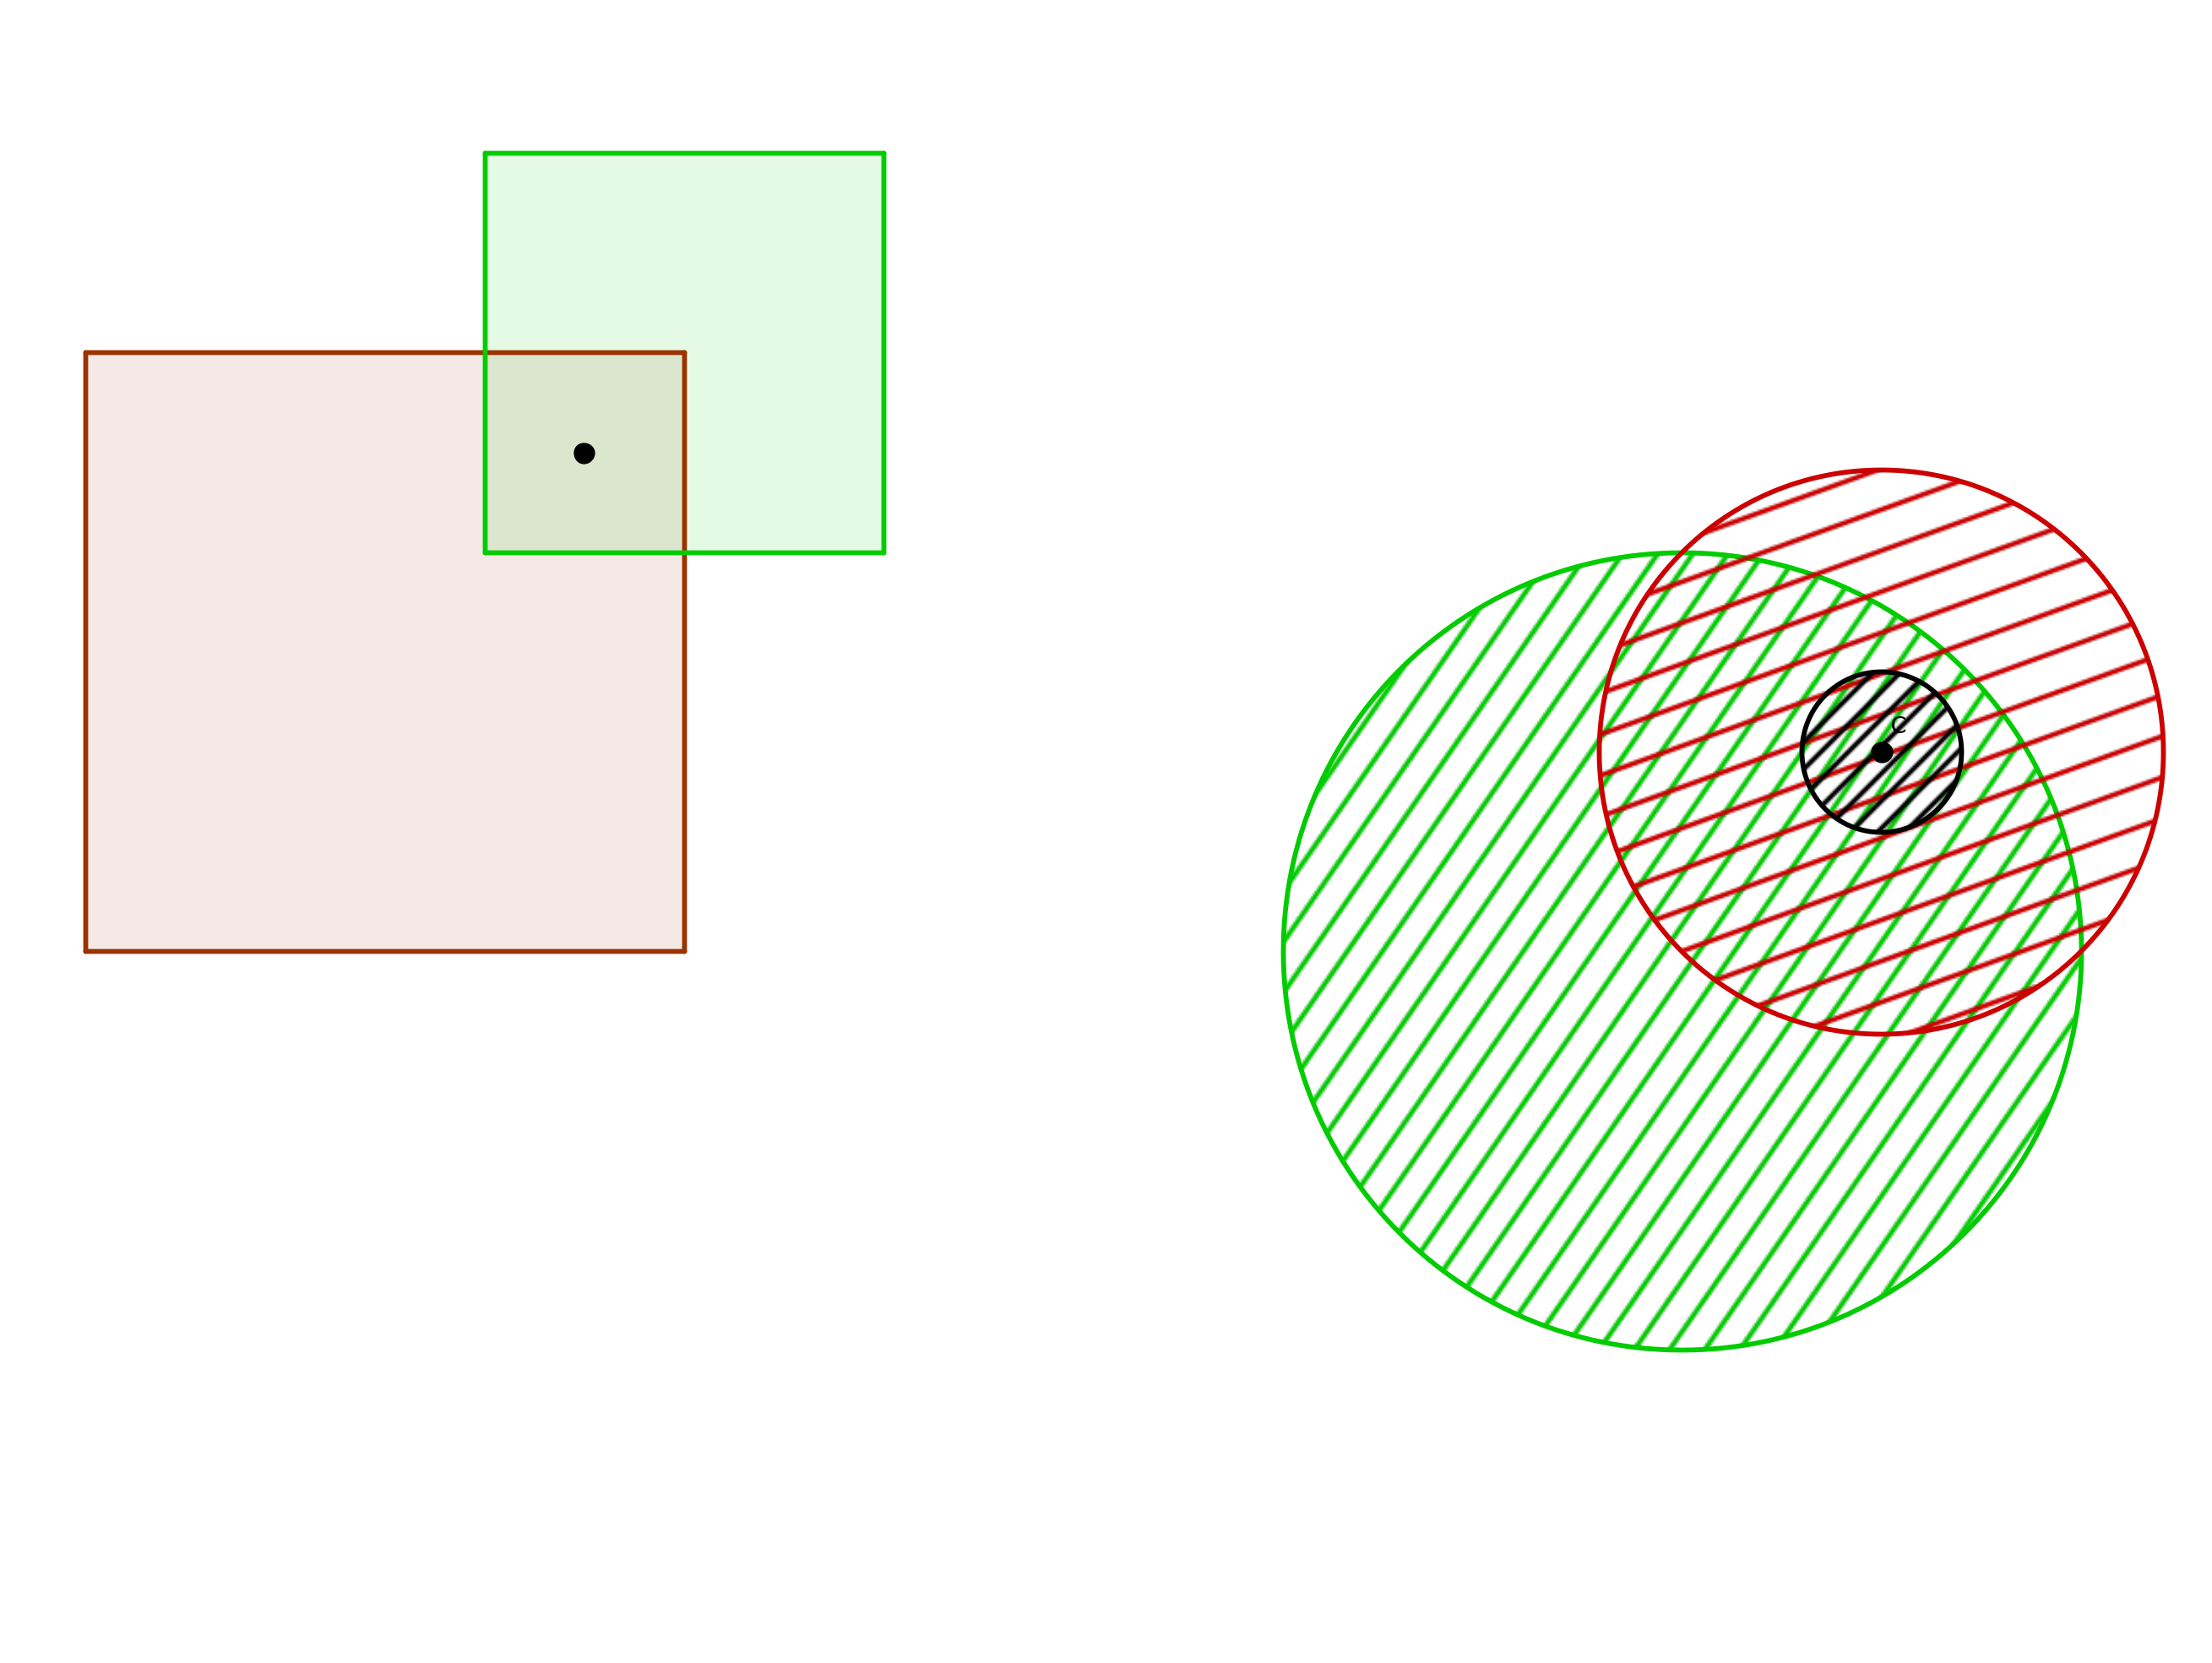
\includegraphics[scale = 0.3]{Figures/Chapter1/basesOfCircularRectangularRegions.png}
    \caption{The basis for $\Bc$ and  $\Bc'$ in  $\R \times \R$  (see example $(2)$).}
    \label{fig_1.2}
\end{figure}

\begin{lemma}\label{1.2.2}
    Let $X$ be a set, and  $\Bc$ be a basis for a topology  $\Tc$ on  $X$. Then 
    $\Tc=\{\bigcup{B}: B \in \Bc\}$.
\end{lemma}
\begin{proof}
    Given a collection $\{B\}$ of basis elements in  $\Bc$, since they are all in  $\Tc$, 
    their unions are also in $\Tc$. Conversely, given  $U \in \Tc$, then for every point 
    $x \in U$, choose a  $B_x \in \B_x$ such that  $x \in B_x \subseteq U$, then  $U=\bigcup_{x \in U}{B_x}$.
\end{proof}

%----------------------------------------------------------------------------------------
%	SECTION 1.3
%----------------------------------------------------------------------------------------

\section{The Order Topology.}

%----------------------------------------------------------------------------------------
%	SECTION 4.3
%----------------------------------------------------------------------------------------

\section{Monotonic Functions and Inverse Functions.}

\begin{definition}
    Let $E \subseteq \R$ be nonempty, and let  $f:E \rightarrow \R$ be a realvalued function. 
    We say that $f$ is \textbf{monotonically increasing} on $E$ if for $x<y$, $f(x) \leq f(y)$. 
    Similarly, $f$ is \textbf{monotonically decreasing} if $f(y) \leq f(x)$. In either case, we call 
    $f$ a \textbf{monotonic} function.
\end{definition}

\begin{example}
    The function $f(x)=x^2$ is not monotonoic on  $I$, but it is monotonically increasing 
    over $[0,\infty)$ and monotonically decreasing over $(-\infty, 0)$. 
\end{example} 

\begin{theorem}\label{4.4.1}
    Suppose that $a, b \in \R$ , with  $a$ and  $b$ distinct, and let  $f$ be contiuous 
    over  $[a,b]$ and differentiable over  $(a,b)$. Then:
        \begin{enumerate}[label=(\arabic*)]
            \item If $f' \geq 0$, for all  $x \in (a,b)$, then $f$ monotonically increasing 
                on $[a,b]$; respectively, if  $f' \leq 0$,  $f$ is monotonically decreasing.

            \item If $f'=0$, for all  $x \in (a,b)$, then $f$ is constant on  $[a,b]$
        \end{enumerate}
\end{theorem}
\begin{proof}
    Assume without loss of generality that $f' \leq 0$, then for any  $a<x_1<x_2<b$, then 
    $f$ is continuous on  $[x_1,x_2]$ and differentiable on $(x_1,x_2)$, hence by the 
    mean value theorem, then there is a $c \in (x_1,x_2)$ such that $f(x_2)f(x_1)=f'(c)(x_2-x_1)$, 
    hence $f(x_2)-f(x_1) \leq 0$, hence $f$ is monotonically decreasing. The case is analogous 
    for  $f'>0$.

    Now suppose that  $f'=0$,  then again by the mean value theorem, there is a  $c \in (x_1,x_2)$ 
    such that $f(x_2)-f(x_1)=f'(c)(x_2-x_1)$, then $f(x_2)-f(x_2)=0$, for $x_1, x_2 \in (a,b)$ 
    arbitrary therefore, $f$ is constant.
\end{proof}

\begin{remark}
    If $f$ and  $g$ are continuous on a nondegenerate inteval,  $[a,b]$, and differentiable 
    on  $(a,b)$, and  $f'=g'$ for all  $x \in (a,b)$, then $f-g$ is constant.
\end{remark}
\begin{proof}
    We repeat the proof for the constant case using the Cauchy mean value theorem; 
    similarly, we can just apply the previous theorem to the function $f-g$.
\end{proof}

Suppose that $f$ is a realvalued function, who has an inverse function  $f^{-1}$. Then 
the graph of  $f^{-1}$ is symmetric to the graph of  $f$ with respect to the line  $y=x$. Then 
visually,  $f^{-1}$ is as smooth as  $f$. Algebraically, we can apply an operation to the graph 
of $f$ to obtain the graph of  $f^{-1}$, and we can observe that smoothness is preserved, however 
we would like to prove this rigorously.

\begin{theorem}\label{4.4.2}
    If $f$ is a  1-1 continuous function of the interval  $I$ onto $\R$, 
    then  $f$ is strictly monotonic on  $I$, and  $f^{-1}$ is continuous and strictly 
    monotonic on $f(I)$.
\end{theorem}
\begin{proof}
    We have that since $f$ is 1-1, then  $f(x)=f(y)$ implies  $x=y$, hence if  $x<y$ 
    are in $I$, then  either $f(x)<f(y)$ or  $f(x)>f(y)$, now if  $f$ is not strictly monotone, then 
    for some $c \in I$, with  $x<c<y$, we have that either  $f(x)$ is inbetween $f(c)$ and  $f(b)$, 
    or  $f(y)$ is between  $f(x)$ and  $f(c)$, hence, by the intermediate value theorem, there is an  $x_1 \in I$ 
    such that $f(x_1)=f(x)$ or $f(x_1)=f(y)$. Then either $x_1=x$ or $x_2=y$ which contradicts the assumption.

    Now suppos that $f$ is strictly increasing on  $I$, since  $f$ is 1-1 ont  $\R$, then 
    $f^{-1}$ exists on  $f(I)$. Now suppose that there are  $y_1,y_2 \in f(I)$ such that 
    $ y_1<y_2$ but $f^{-1}(y_1) \geq f^{-1}(y_2)$, and since $f$ is increasing, then  $f(x_1) \geq f(x_2)$, which 
    is absurd. We also have that $f(I)$ is an interval for if  $I=[a,b]$, then  $f([a,b])=[f(a)f(b)]$ by 
    the intermediate value theorem.

    Now fix  $y_0 \in f(I)$, and let $\epsilon>0$, since $f^{-1}$ is strictly increasing, on $f(I)$ by 
    the above assumption, if $y_0$ is not a right endpoint of $f(I)$, then  $f^{-1}(y_0)$ is not 
    a  right endpoint of  $I$, then  there is an $0<\epsilon_0<\epsilon$ with $\epsilon+\epsilon_0 \in I$. Let  $\delta=f(x_0+\epsilon_0)-f(x_0)$, 
    and suppose that $0<y-y_0<\delta$, then $y_0<y<y_0+\delta=f(x_0+\epsilon_0)$, then since $f^{-1}$ is strictly 
    increasing, it follows that  $x_0<x<x+\epsilon_0$, hence we have that $0<f^{-1}(y)-f^{-1}(y_0)<\epsilon$, 
    that is $f^{-1}(y_0+)$ exists, similatly, if $y_0$ is not a left endpoint of $I$, then  $f^{-1}(y_0-)$ 
    exists. In both cases, we have that $f^{-1}(y_0\pm)=f(y_0)$. Therefore, $f^{-1}$ is contiuous.
\end{proof}

\begin{theorem}[The Inverse Function Theorem]\label{4.4.3}
    Let $f$ be a 1-1 continuous function of an open interval  $I$ onto  $\R$. If  $a \in f(I)$, 
    and if  $f'(f^{-1}(a)) \neq 0$ exists, then  $f^{-1}$ is differentiable at $a$, and 
        \begin{equation}
            (f^{-1})'=\frac{1}{f'}
        \end{equation} 
\end{theorem}
\begin{proof}
    We have that $f(f(^{-1})(x))=x$, if $f$ and $f^{-1}$ are both differentiable, then 
    the chain rule yields the appropriate result. It remains to show that  $f^{-1}$ is 
    differentiable.

    By the previous theorem, we have that  $f$ is strictly monotonic, and say, without 
    loss of generalilty, that  $f$ is strictly increasing. Then  $f^{-1}$ exists, is continuous, and 
    is strictly increasing on $f(I)$. Let  $x_0=f^{-1}(a)$, then there are $c,d \in I$ such that 
    $x_0 \in (c,d) \subseteq I$, thus by the intermediate value theorem, we have that  $f((c,d))=(f(c),f(d))$ which 
    contains  $f(x_0)=a$. Then for $h \neq 0$ sufficiently small  $a+h \in (f(c),f(d))$, 
    hence $f^{-1}(a+h)$ is well defined. Now let  $x=f^{-1}(a+h)$, then  $f(x)=a+h=f(x_0)+h$, 
    thus $h=f(x)-f(x_0)$. Since $f$ is continuous, we have that as  $x \rightarrow x_0$, $h \rightarrow 0$, 
    hence  $x-x_0=f^{-1}(a+h)-f^{-1}(a) \rightarrow 0$, hence $\frac{f^{-1}(a+h)-f^{-1}(a)}{h}=
    \frac{x-x_0}{f(x)-f(x_0)}$ which exists by the continuity of $f$, thus  $f^{-1}$ is differentiable at  $a$.
\end{proof}

\begin{example}
    Take $f(x)=1$ for  $x \in \Q$ and  $f(x)=0$ for  $x \in \com{\R}{\Q}$, which is not 
    continuous at any $x$, also notice that  $x$ is not monotonic.
\end{example}

\begin{lemma}\label{4.4.4}
    Suppose that $f$ is monotonic on  $[a,b]$, if  $x_0 \in [a,b)$, then $f(x_0+)$ exists and 
    $f(x_0) \leq f(x_0+)$ or $f(x_0) \geq f(x_0+)$ (if it is increasing or decreasing respectively). Moreover, 
    if $x_0 \in (a,b]$, then $f(x_0-)$ exists and $f(x_0-) \leq f(x_0)$ or $f(x_0-) \geq f(x_0)$.
\end{lemma}
\begin{proof}
    Fix $x_0 \in [a,b]$, by the symmetry, it suffices to show that $f(x_0-)$ exists and that 
    $f(x_0-) \leq f(x_0)$ if $f$ is increasing. Set  $E=\{f(x):a<x<x_0\}$ and let $s=\sup{E}$. We have 
    $f (x_0)$ is an upeprbound, thus $s$ is finite, and  $s \leq f(x_0)$. It remains to show that $s=f(x_0-)$.

    Now given $\epsilon>0$, by the approximation property, there is an $x_1 \in (a,x_0)$ such that 
    $s-\epsilon<f(x) \leq s$. Since  $f$ is increasing, then we have  $s-\epsilon<f(x_1)<f(x) \leq s$, so 
    choose $\delta=x_0-x_1>0$, then for $-\delta<x-x_0<0$, we have that $|f(x)-s|<\epsilon$, and we are 
    done.
\end{proof}

\begin{theorem}\label{4.4.5}
    If $f$ is monotonic on an interval  $I$, then  $f$ has at most countably many discontinuities on  $I$.
\end{theorem}
\begin{proof}
    Suppose that $f$ is monotonically increasing, without loss of generality. We know that the 
    countable union of atmost countable sets is countable. It suffices to show that the set 
    of all discontinuities of  $f$ is a coutnable union of atmost countable sets.

    Notice that  $\R=\bigcup_{n=1}^{\infty}{[-n,n]}$, now let  $I$ be a closed, bounded, interval  $[a,b]$, 
    and let $E$ be the set of all discontinuities of  $f$ on  $(a,b)$. By lemma \ref{4.4.4}, we have that 
    $f(x-) \leq f(x) \leq f(x+)$, then we see that  $f$ is discontinuous at  $x$ if and only if  $0<f(x+)-f(x-)$. 
    Let  $A_j=\{x \in I: f(x+)-f(x-) \geq \frac{1}{j}\}$, then $A_j \subseteq E$, and we have 
    $E=\bigcup_{j=1}^{\infty}{A_j}$. We would like to show that  $A_j$ is finite for all  $j$.

    For suppose not, then there is a  $j_0$ such that $A_{j_0}$ is infinite, then pick $a \leq x_1<x_2<\dots 
    \leq b\in A_{j_0}$, with $f(x_k+)-f(x_k-)>\frac{1}{j_0}$ for all $k$. Then $f(b)-f(a) \geq f(b)-f(x_1-) 
    \geq f(x_1+)-f(x_1-)>\frac{1}{j_0} \geq f(x_2+)-f(x_1-)=f(x_2+)-f(x_2-)+f(x_2-)-f(x_1-)>\frac{1}{j_0}$, 
    continuing along this line, we get that $f(b)-f(a) \geq \frac{n}{j_0}$ for all $n \geq 1$, which 
    implies that  $f(b)-f(a)$ is infinite, which is a contradiction. Thus  $A_j$ must be finite.
\end{proof}

\begin{figure}
    \centering
    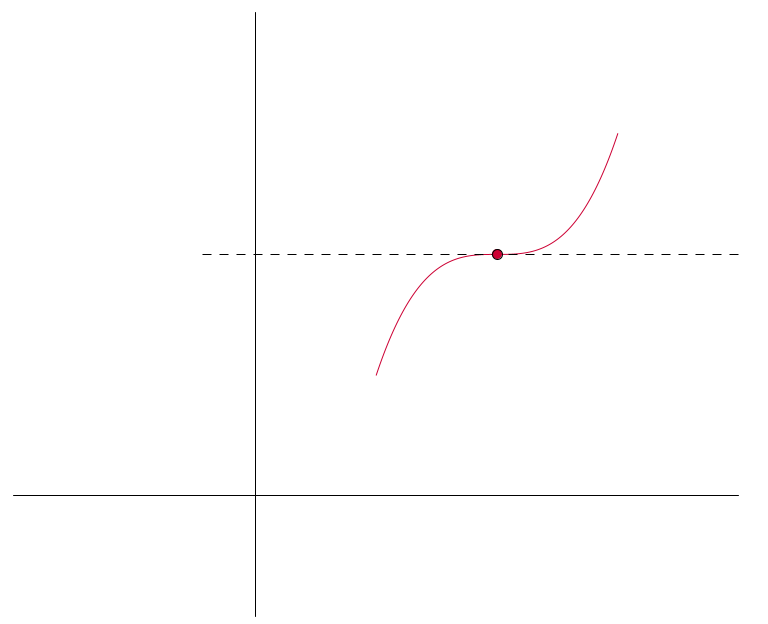
\includegraphics[scale = 0.3]{figures/meanValueDeriv.png}
    \caption{The intermediate value theorem for derviavtives.}
    \label{fig_4.2}
\end{figure}

\begin{theorem}[The Intermediate Value Theorem for Derivatives]\label{4.4.5}
    Suppose that $f$ is differentiable on a closed interval  $[a,b]$, where  $f'(a) \neq g('b)$. If  $y_0 \in \R$ such that $f'(a)<y_0<f'(b)$, then there is an $x_0 \in (a,b)$ such that $f'(x_0)=y_0$.
\end{theorem}
\begin{proof}
    Suppose that $f'(a)<y_0<f'(b)$, now suppose without loss of generality that $f'(a)<f'(b)$. Now let $F(x)=f(x)-y_0x$, for $x \in [a,b]$. We have that $F$ is differentiable on  $(a,b)$, then by the extreme value theorem, $F$ has a local maximum, and a local minumum, let  $F(x_0)$ is a local minimum on $[a,b]$. We have that  $F'(a)=f'(a)-y_0<0$, which is decreasing, so for $h$ sufficiently small, we have  $F(a+h)-F(a)<0$, hence  $F(a)$ cannot be the minumum, hence  $x_0 \neq a$. Similarly,
    $F'(b)=f'(b)-y_0>0$, which is increasing, by similar reasoning, we have that $F(b+h)-F(b)>0$ for  $h$ sufficiently small, hence $F(b)$ cannot be a local maximum, so  $x_0 \neq b$. Thus $x_0 \in (a,b)$. Now since $F(x_0)$ is a local minumum, then we have that $F'(x_0)=0$, hence $f'(x_0)=y_0$
\end{proof}
\begin{remark}
    If in the proof we assume that $f'(a)>y_0>f'(b)$, then we consider $F(x_0)$ to be a local maximum.
\end{remark}

%----------------------------------------------------------------------------------------
%	SECTION 1.1
%----------------------------------------------------------------------------------------

\section{Special Sequences}

\begin{theorem}\label{3.5.1}
    Let $n, p \in \Z^+$. Then the following hold as  $n \rightarrow \infty$.
        \begin{enumerate}[label=(\arabic*)]
            \item $\lim{\frac{1}{n^p}}=0$.

            \item $\lim{\sqrt[p]{n}}=1$.

            \item $\lim{\sqrt[n]{n}}=1$.

            \item If $\alpha \in \R$, then  $\lim{\frac{n^{\alpha}}{(1+p)^n}}=0$.

            \item If $|x|<1$, then  $\lim{x^n}=0$.
        \end{enumerate}
\end{theorem}
\begin{proof}
   \begin{enumerate}[label=(\arabic*)]
       \item Let $n>\sqry[p]{\frac{1}{\epsilon}}$; then $|\frac{1}{n^p}|<\epsilon$.

       \item If $p=1$, we are done. If  $p>1$, let  $x_n=\sqrt[n]{p}-1$, then  $x_n>0$. 
           By the binomial theorem, $1+nx_n \leq (1+x_n)^p=p$, hence $0 \leq x_n \leq \frac{p-1}{p}$. 
           Now if $1>p>0$, then  $ \frac{1}{p}>0$, so we notice that $0 \leq \frac{1}{x_n} \leq \frac{1}{\frac{p-1}{n}}$.

       \item Let $x_n=\sqrt[n]{n}-1$, then  $x_n \geq 0$, then by the binomial theorem again, 
           $n=(1+x_n)^n \geq \frac{n(n-1)}{2}x_n^2$, then $0 \leq x_n \leq \sqrt{\frac{2}{n-1}}$.

       \item Let $k \in \Z^+$ such that  $k>\alpha$. Then  $n>2k$,let  $(1+p)^n> {n \choose k}p^k>
           \frac{n^kp^k}{2^kk!}$. So $0<\frac{n^{\alpha}}{(1+p)^n}<\frac{2^kk!}{p^k}n^{\alha-k}$, since 
           $\alpha-k<0$,  $n^{\alpha-k} \rightarrow 0$ and we are done.

       \item Take  $\alpha=0$, and let  $x=\frac{1}{1+p}$, then the result follow.
   \end{enumerate} 		
\end{proof}


%----------------------------------------------------------------------------------------
%	CHAPTER 2
%----------------------------------------------------------------------------------------

\chapter{The Real Numbers.} % Main chapter title

\label{Chapter1} % Change X to a consecutive number; for referencing this chapter elsewhere, use \ref{ChapterX}

%% to include section files use the \input{} command.

%----------------------------------------------------------------------------------------
%	SECTION 3.1
%----------------------------------------------------------------------------------------

\section{Some Elementary Observations} \hspace{10mm}

Consider the equation $x^2-117x+31=0$. We claim that there are no integer solutions to this equation. Let $n$ be an integer
, then $n$ is either even or odd. If $n$ is even, then so is  $n^2$ and  $17n$; hence $x^2-117x+31$ is odd. Likewise if $n$ 
is odd, then so is $n^2$ and  $117n$, thus $x^2-117x+31$ is even and so we see that $x^2-117x+31$ is never $0$.  

%----------------------------------------------------------------------------------------
%	SECTION 1.2
%----------------------------------------------------------------------------------------

\section{The Basis and Subbasis for a Topology.}

\begin{definition}
    If $X$ is a set, the \textbf{basis} for a topology on $X$ is a collection $\Bc$ of 
    subsets of  $X$, called \textbf{basis elements}, such that:
        \begin{enumerate}[label=(\arabic*)]
            \item For every $x \in X$, there is a  $B \in \Bc$ such that $x \in B$.

            \item For $B_1,B_2 \in \Bc$, if $x \in B_1 \cap B_2$, then there is a $B_3 \in \Bc$ 
                such that $x \in B_3 \subseteq B_1 \cap B_2$
        \end{enumerate}
We define the topology $\Tc$ \textbf{generated} by $\Bc$ to be collection of open sets: 
$\Tc=\{U \subseteq X: x \in B \text{ for some } B \in \Bc\}$.
\end{definition}

\begin{theorem}\label{1.2.1}
    Let $X$ be a set, and  $\Bc$ a basis of  $X$, then the collection of subsets 
    of  $X$, $\Tc=\{U \subseteq X: x \in B \text{ for some } B \in \Bc\}$ is a topology on $X$.
\end{theorem}
\begin{proof}
    Let $\Bc$ be a basis for a topology in  $X$, and consider  $\Tc$ as defined 
    above. Cleary, $\emptyset \in X$ and so is  $X$.

    Now let  $\{U_{\alpha}\}$ be a subcollection of subsets of  $X$, and let  $U=\bigcup{U_{\alpha}}$. 
    Then if  $x \in U$ for some  $\alpha$, there is a  $B_{\alpha}$ such that  $x \in B_{\alpha} \subseteq U_{\alpha}$, 
    thus  $x \in B_{\alpha} \subseteq U$.

    Now let  $x \in  U_1 \cap U_2$, and choose $B_1,B_2 \in \Bc$ such that $x \in B_1 \subseteq U_1$ 
    and $x \in B_2 \subseteq U_2$. Then  by definition, there is a $B_3$ for which $x \in B_3 \subseteq B_1 \cap B_2$.
    Now suppose for arbitrary $n$, that  $U=\bigcap_{i=1}^{n}{U_i} \in \Tc$, for some finite 
    subcollection  $\{U_i\}$ of subsets of  $X$. Then by let  $B_n, B_{n+1} \in \Bc$ such that 
    $x \in B_n \subseteq U$ and  $x \in B_{n+1} \subseteq U_{n+1}$. Then by our hypothesis, there is a  $B$ 
for which  $x \in B \subseteq B_n \cap B_{n+1}$, thus  $U \cap U_{n+1}=\bigcap_{i=1}^{n+1}{U_i} \in \Tc$. 
This make $\Tc$ a topology on  $X$.
\end{proof}

\begin{example}
    \begin{enumerate}[label=(\arabic*)]
        \item Let $\Bc$ be the set of all circular regions in the plane  $\R \times \R$, then 
            $\Bc$ satisfies the conditions needed for a basis.

        \item The collection  $\Bc'$ in  $\R \times \R$ of all rectangular region also 
            forms a basis for a topology on  $\R \times \R$.

        \item For any set  $X$, the set of all  $1$-point elements of  $X$ forms a 
            basis for a topology on  $X$.
    \end{enumerate}		
\end{example}

\begin{figure}
    \centering
    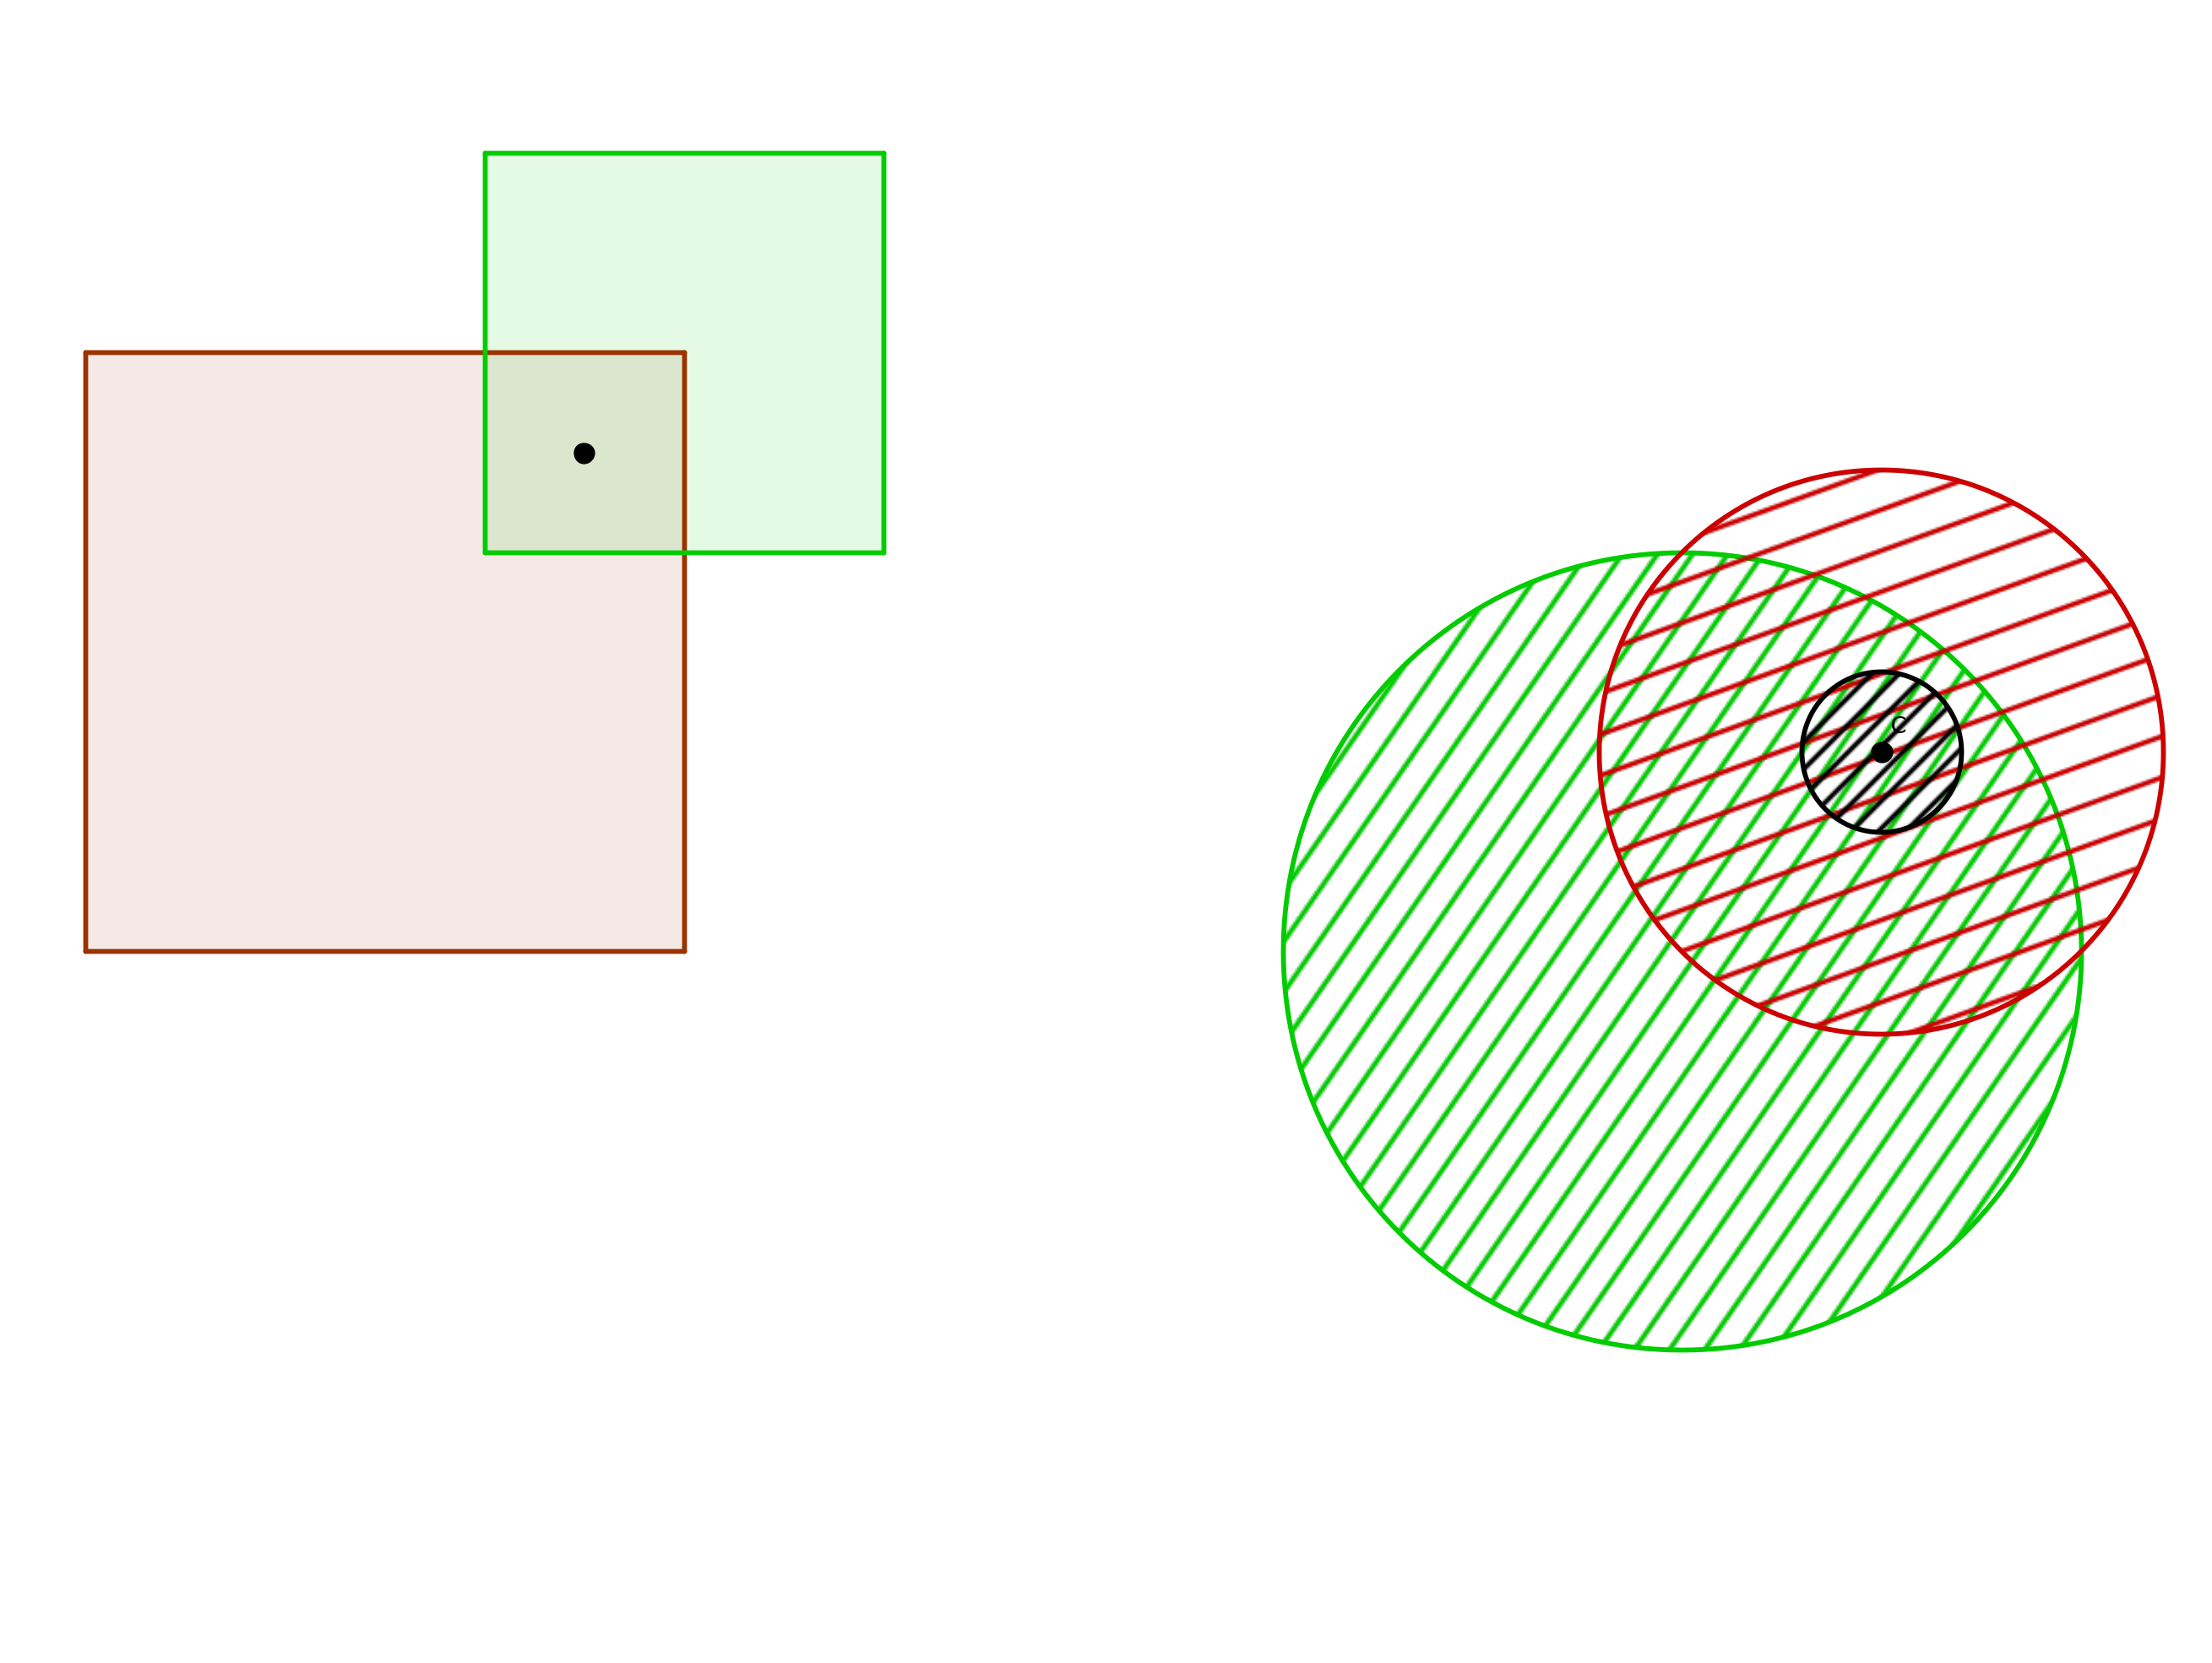
\includegraphics[scale = 0.3]{Figures/Chapter1/basesOfCircularRectangularRegions.png}
    \caption{The basis for $\Bc$ and  $\Bc'$ in  $\R \times \R$  (see example $(2)$).}
    \label{fig_1.2}
\end{figure}

\begin{lemma}\label{1.2.2}
    Let $X$ be a set, and  $\Bc$ be a basis for a topology  $\Tc$ on  $X$. Then 
    $\Tc=\{\bigcup{B}: B \in \Bc\}$.
\end{lemma}
\begin{proof}
    Given a collection $\{B\}$ of basis elements in  $\Bc$, since they are all in  $\Tc$, 
    their unions are also in $\Tc$. Conversely, given  $U \in \Tc$, then for every point 
    $x \in U$, choose a  $B_x \in \B_x$ such that  $x \in B_x \subseteq U$, then  $U=\bigcup_{x \in U}{B_x}$.
\end{proof}

%%----------------------------------------------------------------------------------------
%	SECTION 1.3
%----------------------------------------------------------------------------------------

\section{The Order Topology.}





%\bibliographystyle{abbrv}
%\bibliography{references}

\end{document}
